\documentclass[
    iai, % Saisir le nom de l'institut rattaché
    eai, % Saisir le nom de l'orientation
    confidential, % Décommentez si le travail est confidentiel
]{heig-tb}

\usepackage[nooldvoltagedirection,european,americaninductors]{circuitikz}
\usepackage{float}

\signature{mbernasconi.svg} % Remplacer par votre propre signature vectorielle.

\makenomenclature
\makenoidxglossaries
\makeindex

\addbibresource{bibliography.bib}

\input{nomenclature}
\input{acronyms}
\newglossaryentry{heig-vd}{
    name=HEIG-VD,
    description={Haute École d'Ingénierie et de Gestion du canton de Vaud}
}
\newglossaryentry{hes-so}{
    name=HES-SO,
    description={Haute École Supérieure de Suisse Occidentale}
}
\newglossaryentry{latex}{
    name=latex,
    description={Un langage et un système de composition de documents}
}
\newglossaryentry{maths}{
    name=mathematics,
    description={Les mathematiques sont ce que les mathématiciens fonts}
}
\newglossaryentry{tem00}{
    name=TEM\textsubscript{00},
    description={Ce mode, également appelé mode fondamental gaussien, est un concept clé en physique, notamment en optique et en technologie laser. TEM signifie Transverse Électromagnétique, et les chiffres “00” indiquent l'ordre du mode. Ce mode se caractérise par un profil d'intensité gaussien, symétrique par rapport à l'axe du faisceau, dont l'intensité diminue de manière exponentielle du centre vers les bords. \cite{modeTEM00}}
}
% Auteur du document (étudiant-e) en projet de Bachelor
\author{Samuel Rechsteiner}

% Activer l'option pour l'accord du féminin dans le texte
\genre{male}

% Titre de votre travail de Bachelor
\title{Pinces optiques pour pick-and-place de microobjets}

% Le sous titre est optionnel
\subtitle{Travail de Bachelor}

% Nom du professeur responsable
\teacher {Prof. Dr. S. Schintke (HEIG-VD)}

% Mettre à jour avec la date de rendu du travail
\date{\today}

% Numéro de TB
\thesis{7212}



\surroundwithmdframed{minted}

%% Début du document
\begin{document}
\selectlanguage{french}
\maketitle
\frontmatter
\clearemptydoublepage

%% Requis par les dispositions générales des travaux de Bachelor
\preamble
\authentification

%% Résumé / Résumé publiable / Version abrégée
\begin{abstract}
    % Francais
Les pinces optiques sont des dispositifs basés sur l'utilisation d'un faisceau laser focalisé permettant de piéger et de manipuler des objets microscopiques, tels que des microbilles. Le système exploite la force de gradient générée par la focalisation de la lumière, qui attire les particules au centre du laser.

Ce projet de bachelor consiste à mettre en service un système de pinces optiques, à passer d'un système de sécurité laser de classe 3B (port de lunettes de protection obligatoire) à un système sécurisé de classe 1 (aucune protection requise), afin de permettre son utilisation en toute sécurité par des utilisateur\(\cdot\)trices non-expert\(\cdot\)es. Le projet inclut également la création d'une notice de laboratoire simple et claire, proposant des expériences à réaliser avec le système, ainsi que le développement d'une application regroupant toutes les fonctionnalités nécessaires pour piloter et exploiter l'ensemble du dispositif.

Le projet a été réalisé au Laboratoire d'Applications des NanoSciences (COMATEC-LANS) à la HEIG-VD. La sécurisation du dispositif a été effectuée en ajoutant des protections mécaniques, un boîtier avec bouton d'arrêt d'urgence, ainsi que des capteurs électriques associés aux protections : lorsqu'elles sont ouvertes, ces capteurs interrompent automatiquement l'alimentation du laser. Un bouton à clé de maintenance a également été câblé. Lorsqu'il est activé, il permet d'effectuer des réglages sur les différents composants tout en gardant le laser allumé (le port des lunettes de protection est alors obligatoire).

En conclusion, le système de pinces optiques a été pris en main, sécurisé et rendu accessible pour un usage pour des utilisateur\(\cdot\)trices non-expert\(\cdot\)es. Une documentation claire a été créée pour accompagner les utilisateur\(\cdot\)trices, et une interface logicielle intuitive permet de piloter le système de manière simple et complète.

% \asterism

% English
% Optical tweezers are devices based on the use of a focused laser beam to trap and manipulate microscopic objects, such as microbeads. The system exploits the gradient force generated by focusing the light, which attracts the particles to the centre of the laser.

% This Bachelor's project involves commissioning a system of optical tweezers, upgrading it from a class 3B laser safety system (protective glasses must be worn) to a class 1 safety system (no protection required), so that it can be used safely by non-expert users. The project also includes the creation of a simple and clear laboratory manual, proposing experiments to be carried out with the system, as well as the development of an application bringing together all the functions needed to control and operate the entire device.

% The project was carried out at the NanoSciences Applications Laboratory (COMATEC-LANS) at HEIG-VD. The device was made safe by adding mechanical protections, a box with an emergency stop button, and electrical sensors associated with the protections: when they are open, these sensors automatically interrupt the laser's power supply. A key-operated maintenance button has also been wired in. When activated, it enables adjustments to be made to the various components while the laser is still switched on (protective goggles must be worn).

% In conclusion, the optical tweezers system was taken in hand, secured and made accessible for use by non-expert users. Clear documentation has been created to assist users, and an intuitive software interface makes it simple and comprehensive to control the system.
\end{abstract}

%% Sommaire et tables
\clearemptydoublepage
{
    \tableofcontents
    \let\cleardoublepage\clearpage
    \listoffigures
    \let\cleardoublepage\clearpage
    \listoftables
    \let\cleardoublepage\clearpage
    \listoflistings
}

\printnomenclature
\clearemptydoublepage
\pagenumbering{arabic}

%% Contenu
\mainmatter
\chapter{Introduction}
L'introduction est une section requise dans un rapport technique. Introduisez votre travail, l'idée de départ et les objectifs attendus. Un lecteur qui découvrirait votre projet au travers de cette introduction devrait ainsi être capable d'en comprendre le cadre, l'idée générale et les aboutissants du projet.

Le but de ce projet de bachelor consiste, premièrement, d'apporter plus de sécurité au système de pinces optiques par laser afin de faciliter son utilisation au quotidien. Deuxièmement, une proposition d'expérience avec un mode d'emploi compact est proposé pour le cours de NANO pour les systèmes industriels.Troisièmement, des tests de déplacements de microbilles dans différents milieux, de différentes viscosités, dans différents types de réservoirs ainsi que de multiples canaux.
\newpage
\section{Contexte}

Le kit de pinces optiques portables, Portable Optical Tweezers, est un dispositif qui permet de déplacer de microobjets grâce à un faisceau laser focalisé. L'entreprise qui fabrique ce kit, Thorlabs, est une entreprise américaine qui conçoit des composants optiques, des lasers, des instruments de mesure.

L'image ci-dessous (voir Figure \ref{chemin_laser_caméra}) montre le trajet parcouru par le laser (\textcolor{red}{en rouge}), ainsi que du microscope vers la caméra (\textcolor[RGB]{0, 120, 0}{en vert}).

\begin{figure}[H]
    \begin{center}
        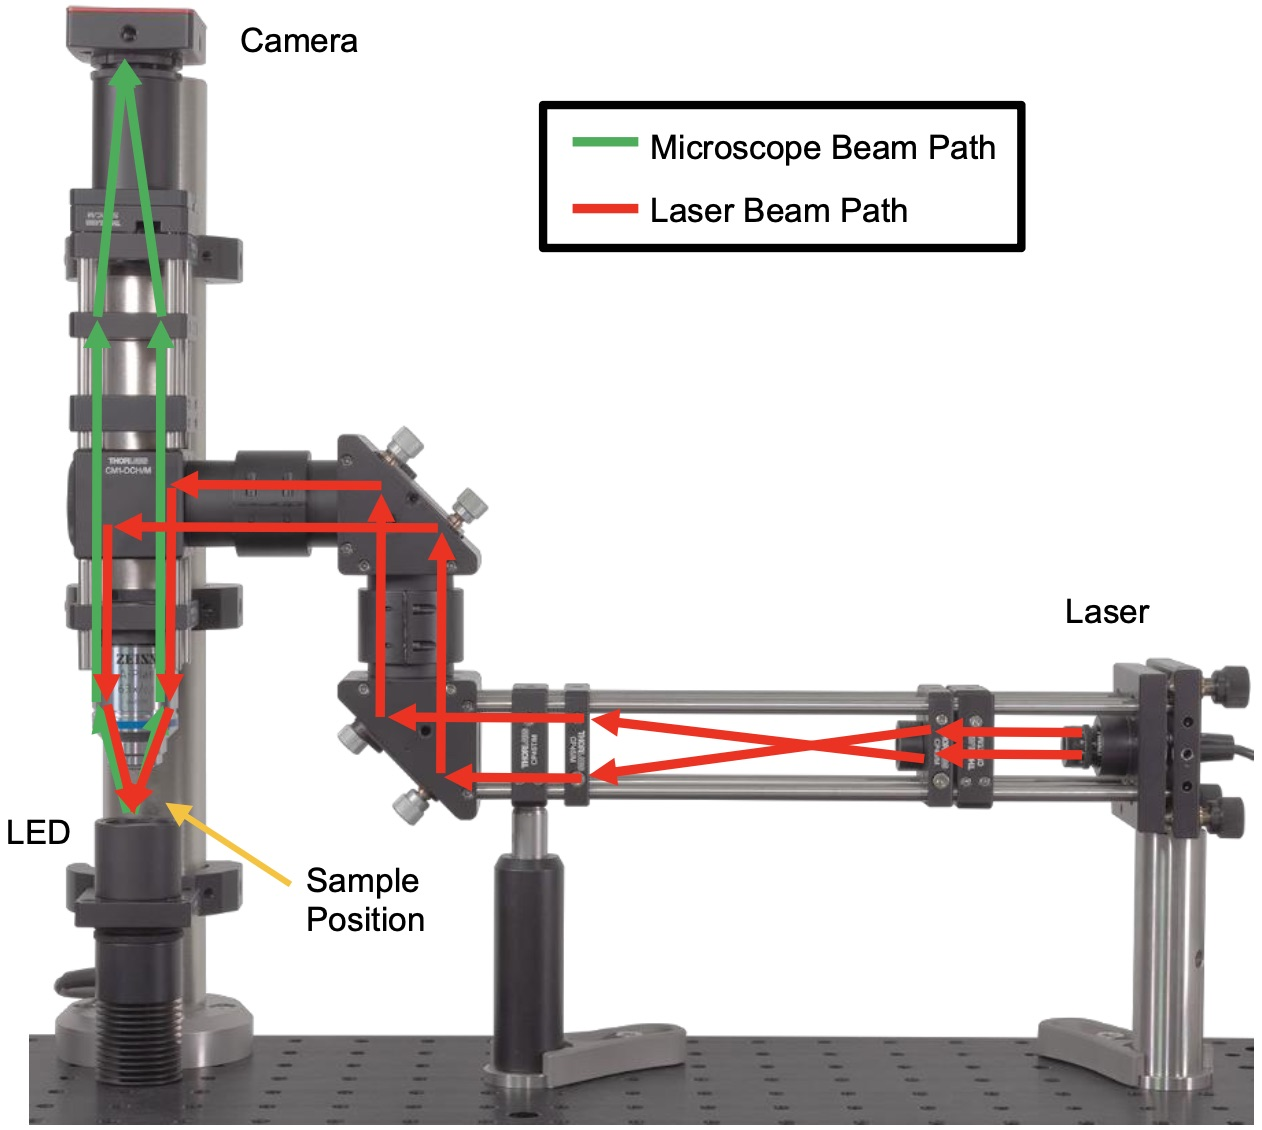
\includegraphics[width=0.7\textwidth]{assets/figures/Introduction/chemin_laser_camera.jpeg}
    \end{center}
    \caption{Trajet du laser et du microscope}
    \label{chemin_laser_caméra}
\end{figure}

La figure ci-dessous (voir Figure \ref{kit_vierge}) correspond au kit reçu lors du premier jour de TB. Le kit a été monté par un assistant du laboratoire COMATEC-LANS.

\begin{figure}[H]
    \begin{center}
        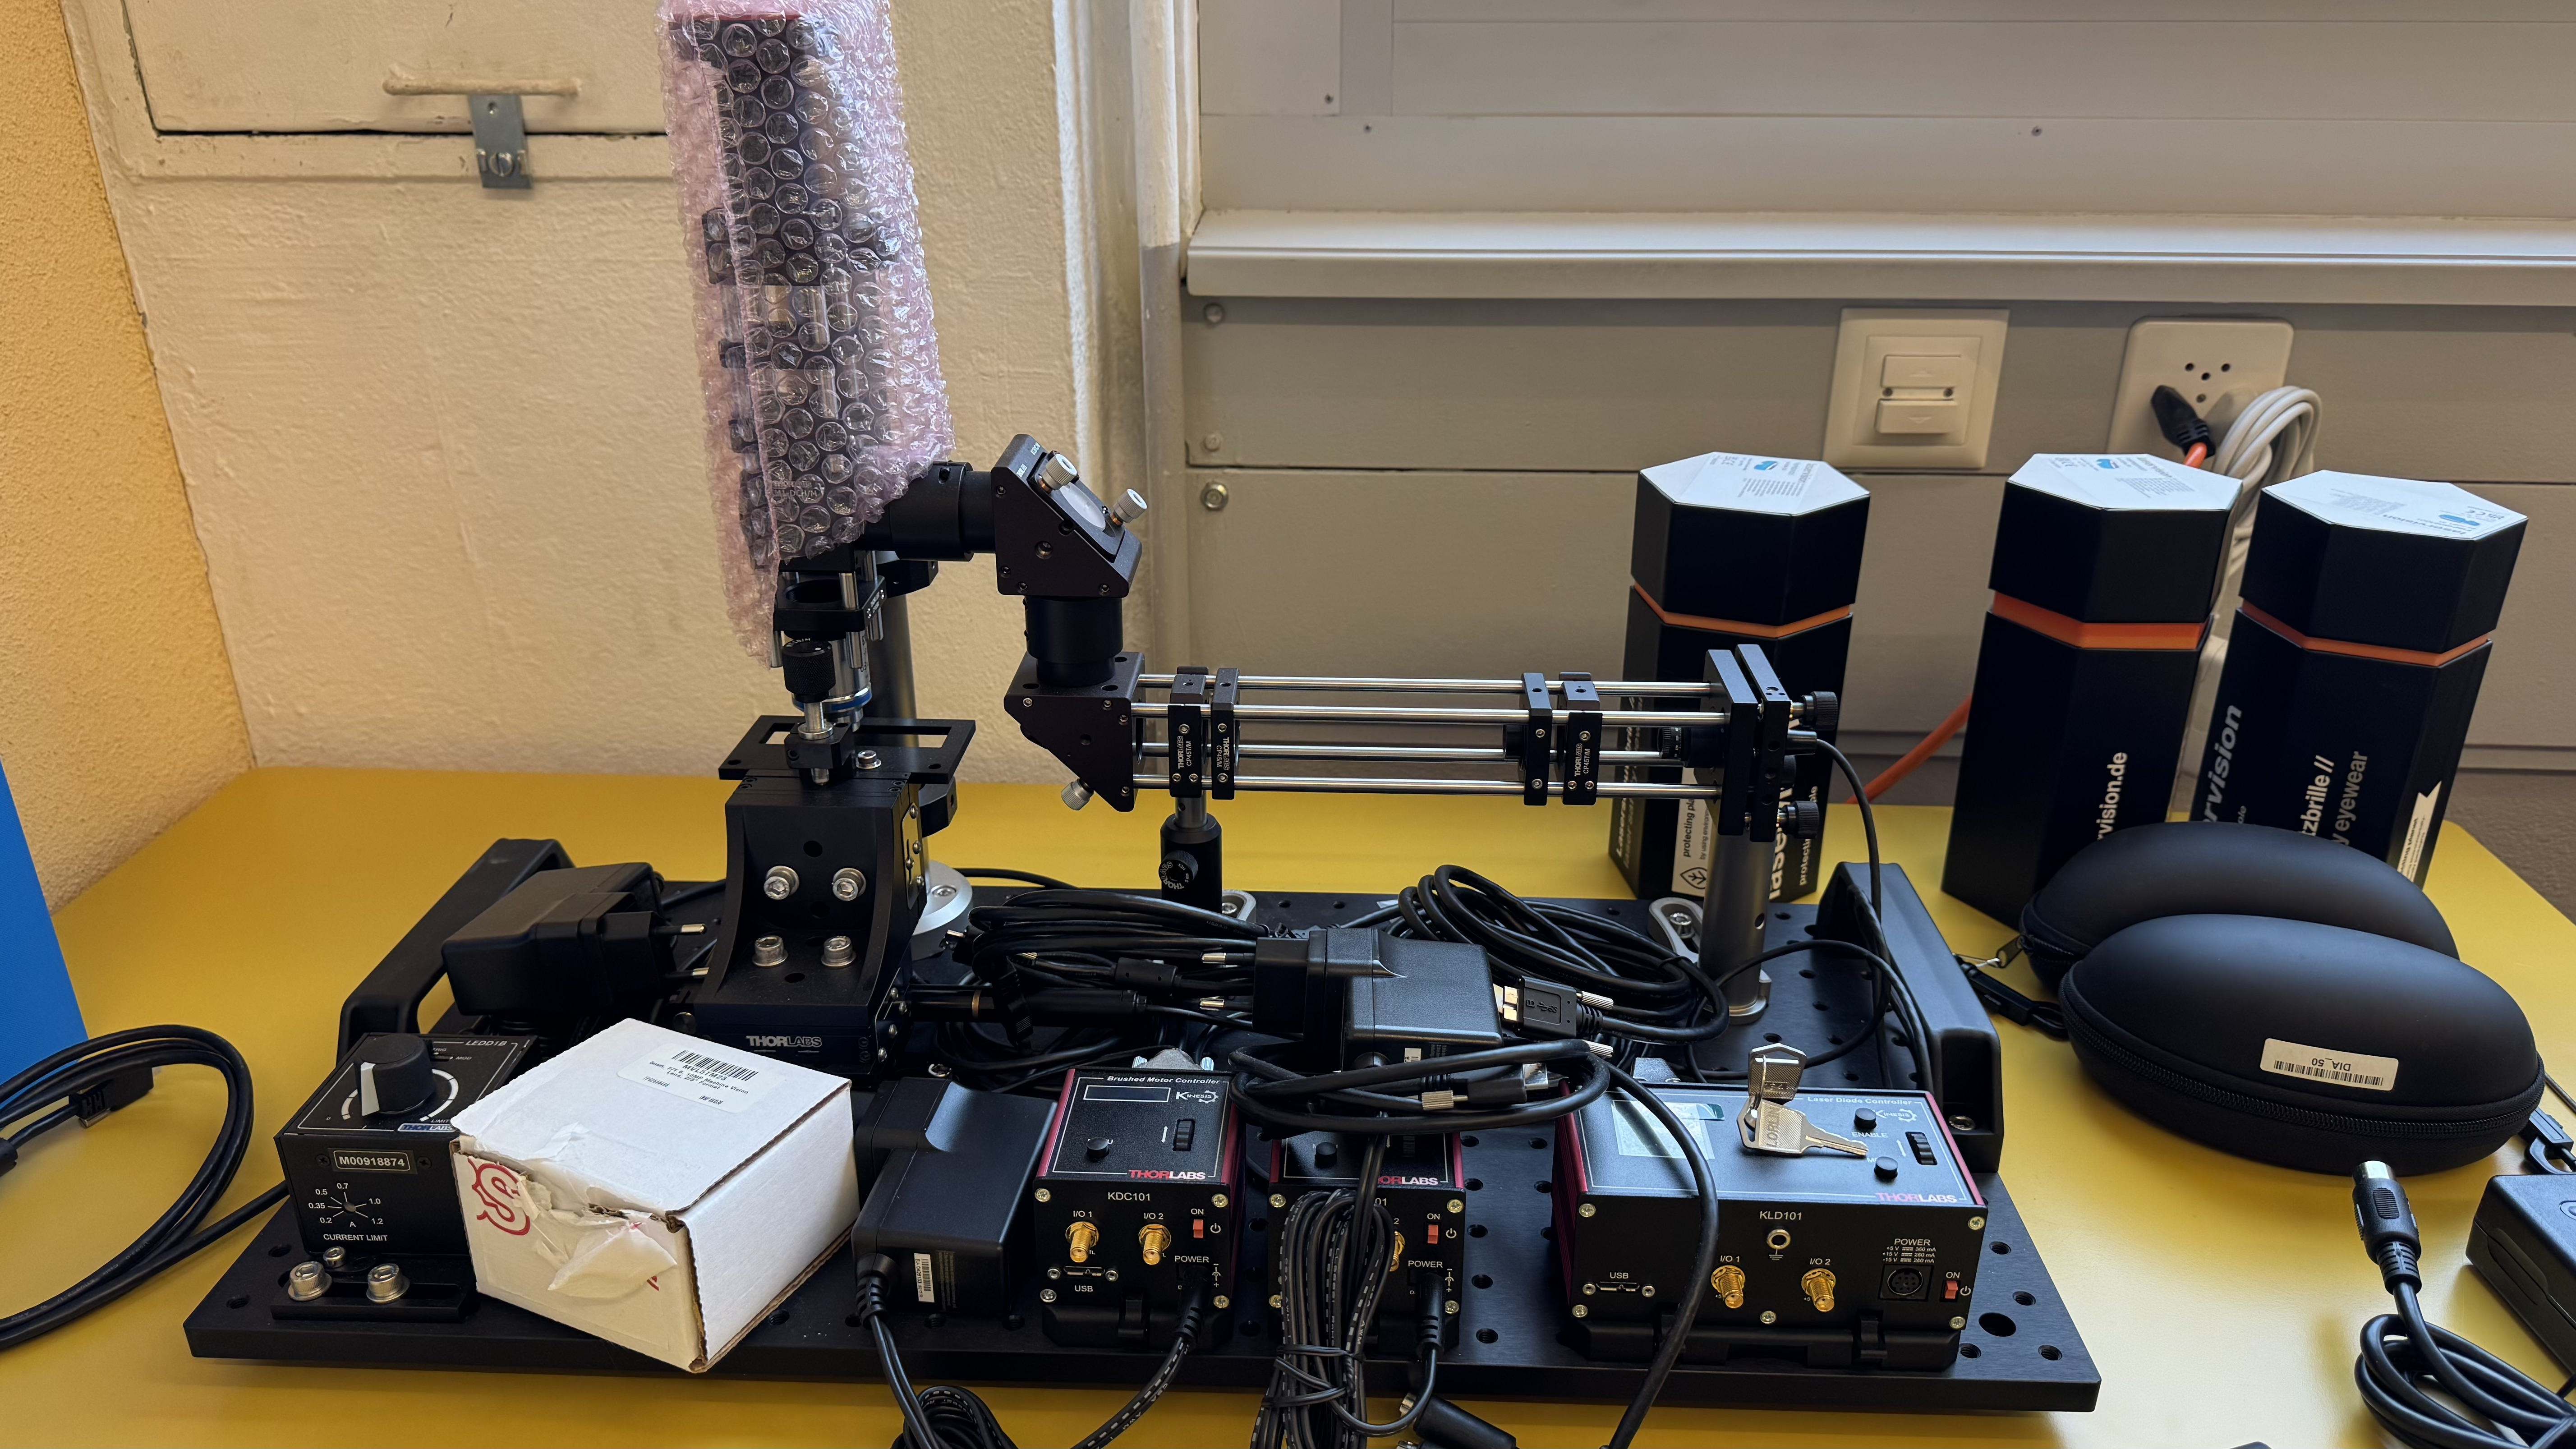
\includegraphics[width=0.7\textwidth]{assets/figures/Introduction/kit_vierge.jpeg}
    \end{center}
    \caption{Kit Portable Optical Tweezers de Thorlabs}
    \label{kit_vierge}
\end{figure}

\newpage
Une représentation 3D du kit, accompagnée de légendes pour chaque composant, a été réalisé par mes soins. Ce modèle CAO permet une clareté et une compréhension plus rapide des différents éléments. Les différentes modélisations 3D des composants ont directement été pris du site Thorlabs \cite{noauthor_portable_nodate}, dans l'onglet \guillemotleft Component List\guillemetright. Je me suis chargé de les rassembler dans un seul fichier CAO et de faire l'assemblage (voir Figure \ref{kit_CAO_vierge_annote}).

\begin{figure}[H]
    \begin{center}
        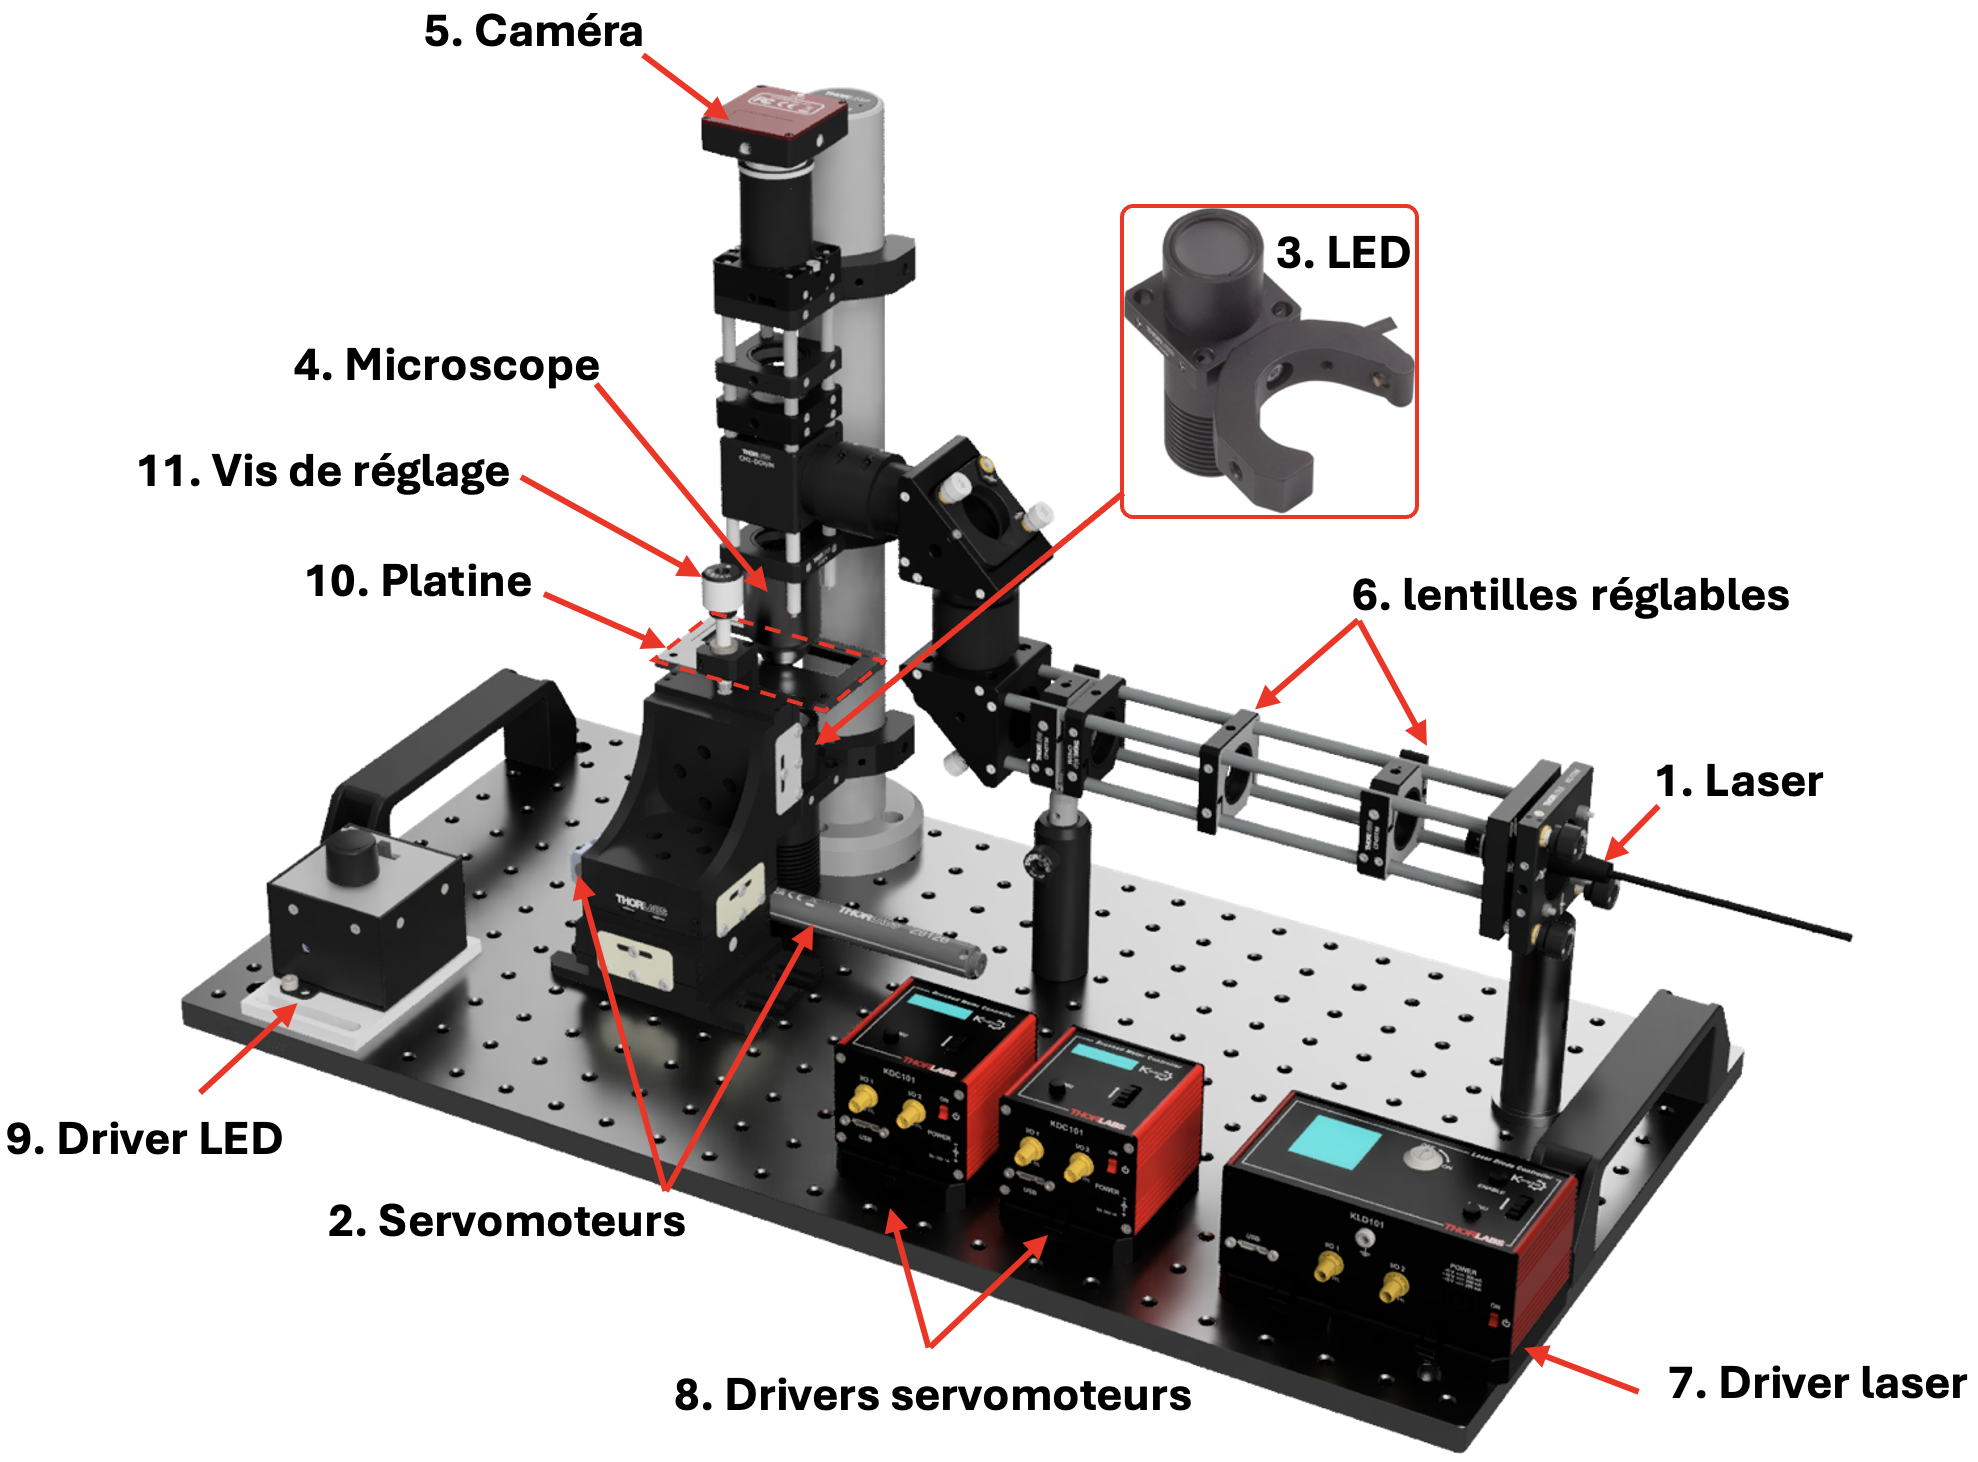
\includegraphics[width=\textwidth]{assets/figures/Introduction/Kit_CAO_vierge_annote.png}
    \end{center}
    \caption{CAO du kit avec annotations des principaux composants}
    \label{kit_CAO_vierge_annote}
\end{figure}

\begin{enumerate}
    \item Laser d'une longueur d'onde 658 nm (couleur rouge visible) avec une puissance maximale de 40 mW.
    \item Les servomoteurs permettent de déplacer la platine en X Y.
    \item La LED permet un réglage manuel de l'éclairage.
    \item Microscope équipé d'un objectif avec un grossissement de $63\times$ et une ouverture numérique de 0,8.
    \item Caméra couleur de 1,6 mégapixel.
    \item Lentilles réglables pour modifier la hauteur de la mise au point du laser.
    \item Ce driver permet de piloter le laser, soit directement avec les boutons intégrés, soit via l'application Kinesis pour une meilleure ergonomie.
    \item Ces driver permettent le pilotage des servomoteurs, soit directement avec les boutons intégrés, soit via l'application Kinesis pour une meilleure ergonomie.
    \item Ce driver permet de faire varier l'intensité lumineuse de la LED.
    \item La platine permet d'accueillir l'échantillon que l'on veut analyser.
    \item La vis de réglage, de pas très fin, permet d'ajuster précisement la hauteur souhaitée de la platine.
\end{enumerate}

\section{Objectifs}

Les différents objectifs de ce travail de bachelor sont listés ci-dessous :
\begin{enumerate}
    \item Mettre en service le kit : câblage, calibration du laser
    \item Conception de protection contre le laser afin d'apporter plus de sécurité lors de l'utilisation du kit
    \item Élaboration d'une notice de laboratoire compacte pour utiliser simplement le kit
    \item Effectuer des tests de déplacements de microbilles dans différents milieux, de différentes viscosités, dans différents types de réservoirs ainsi que de multiples canaux.
    \item Analyses expérimentales des forces de déplacement en fonction de la viscosité des fluides
\end{enumerate}

\subsection{Mise en service du kit}

La première partie consiste à mettre en service le kit. Il faut alimenter les différents drivers qui contrôlent les moteurs, la LED ainsi que le driver pour le laser. Viens ensuite la procédure de calibration du laser, ainsi que l'installation des logiciels permettant de contrôler, d'une part les drivers des moteurs, et d'autre part le driver du laser.
\subsection{Protections contre le laser}
La deuxième partie porte sur la conception des protections contre le laser. Deux parties du kit ont besoin d'avoir une protection totale afin d'éviter toutes reflexions nocives du laser dans les yeux de l'utilisateur. La première protection à réaliser est située au début du laser et va devoir entouré toute la cage oû le laser passe (voir Figure \ref{protection_laser_début}). L'encadré en \textcolor{red}{rouge} représente l'endroit où va devoir être imaginer la protection.

\begin{figure}[H]
    \begin{center}
        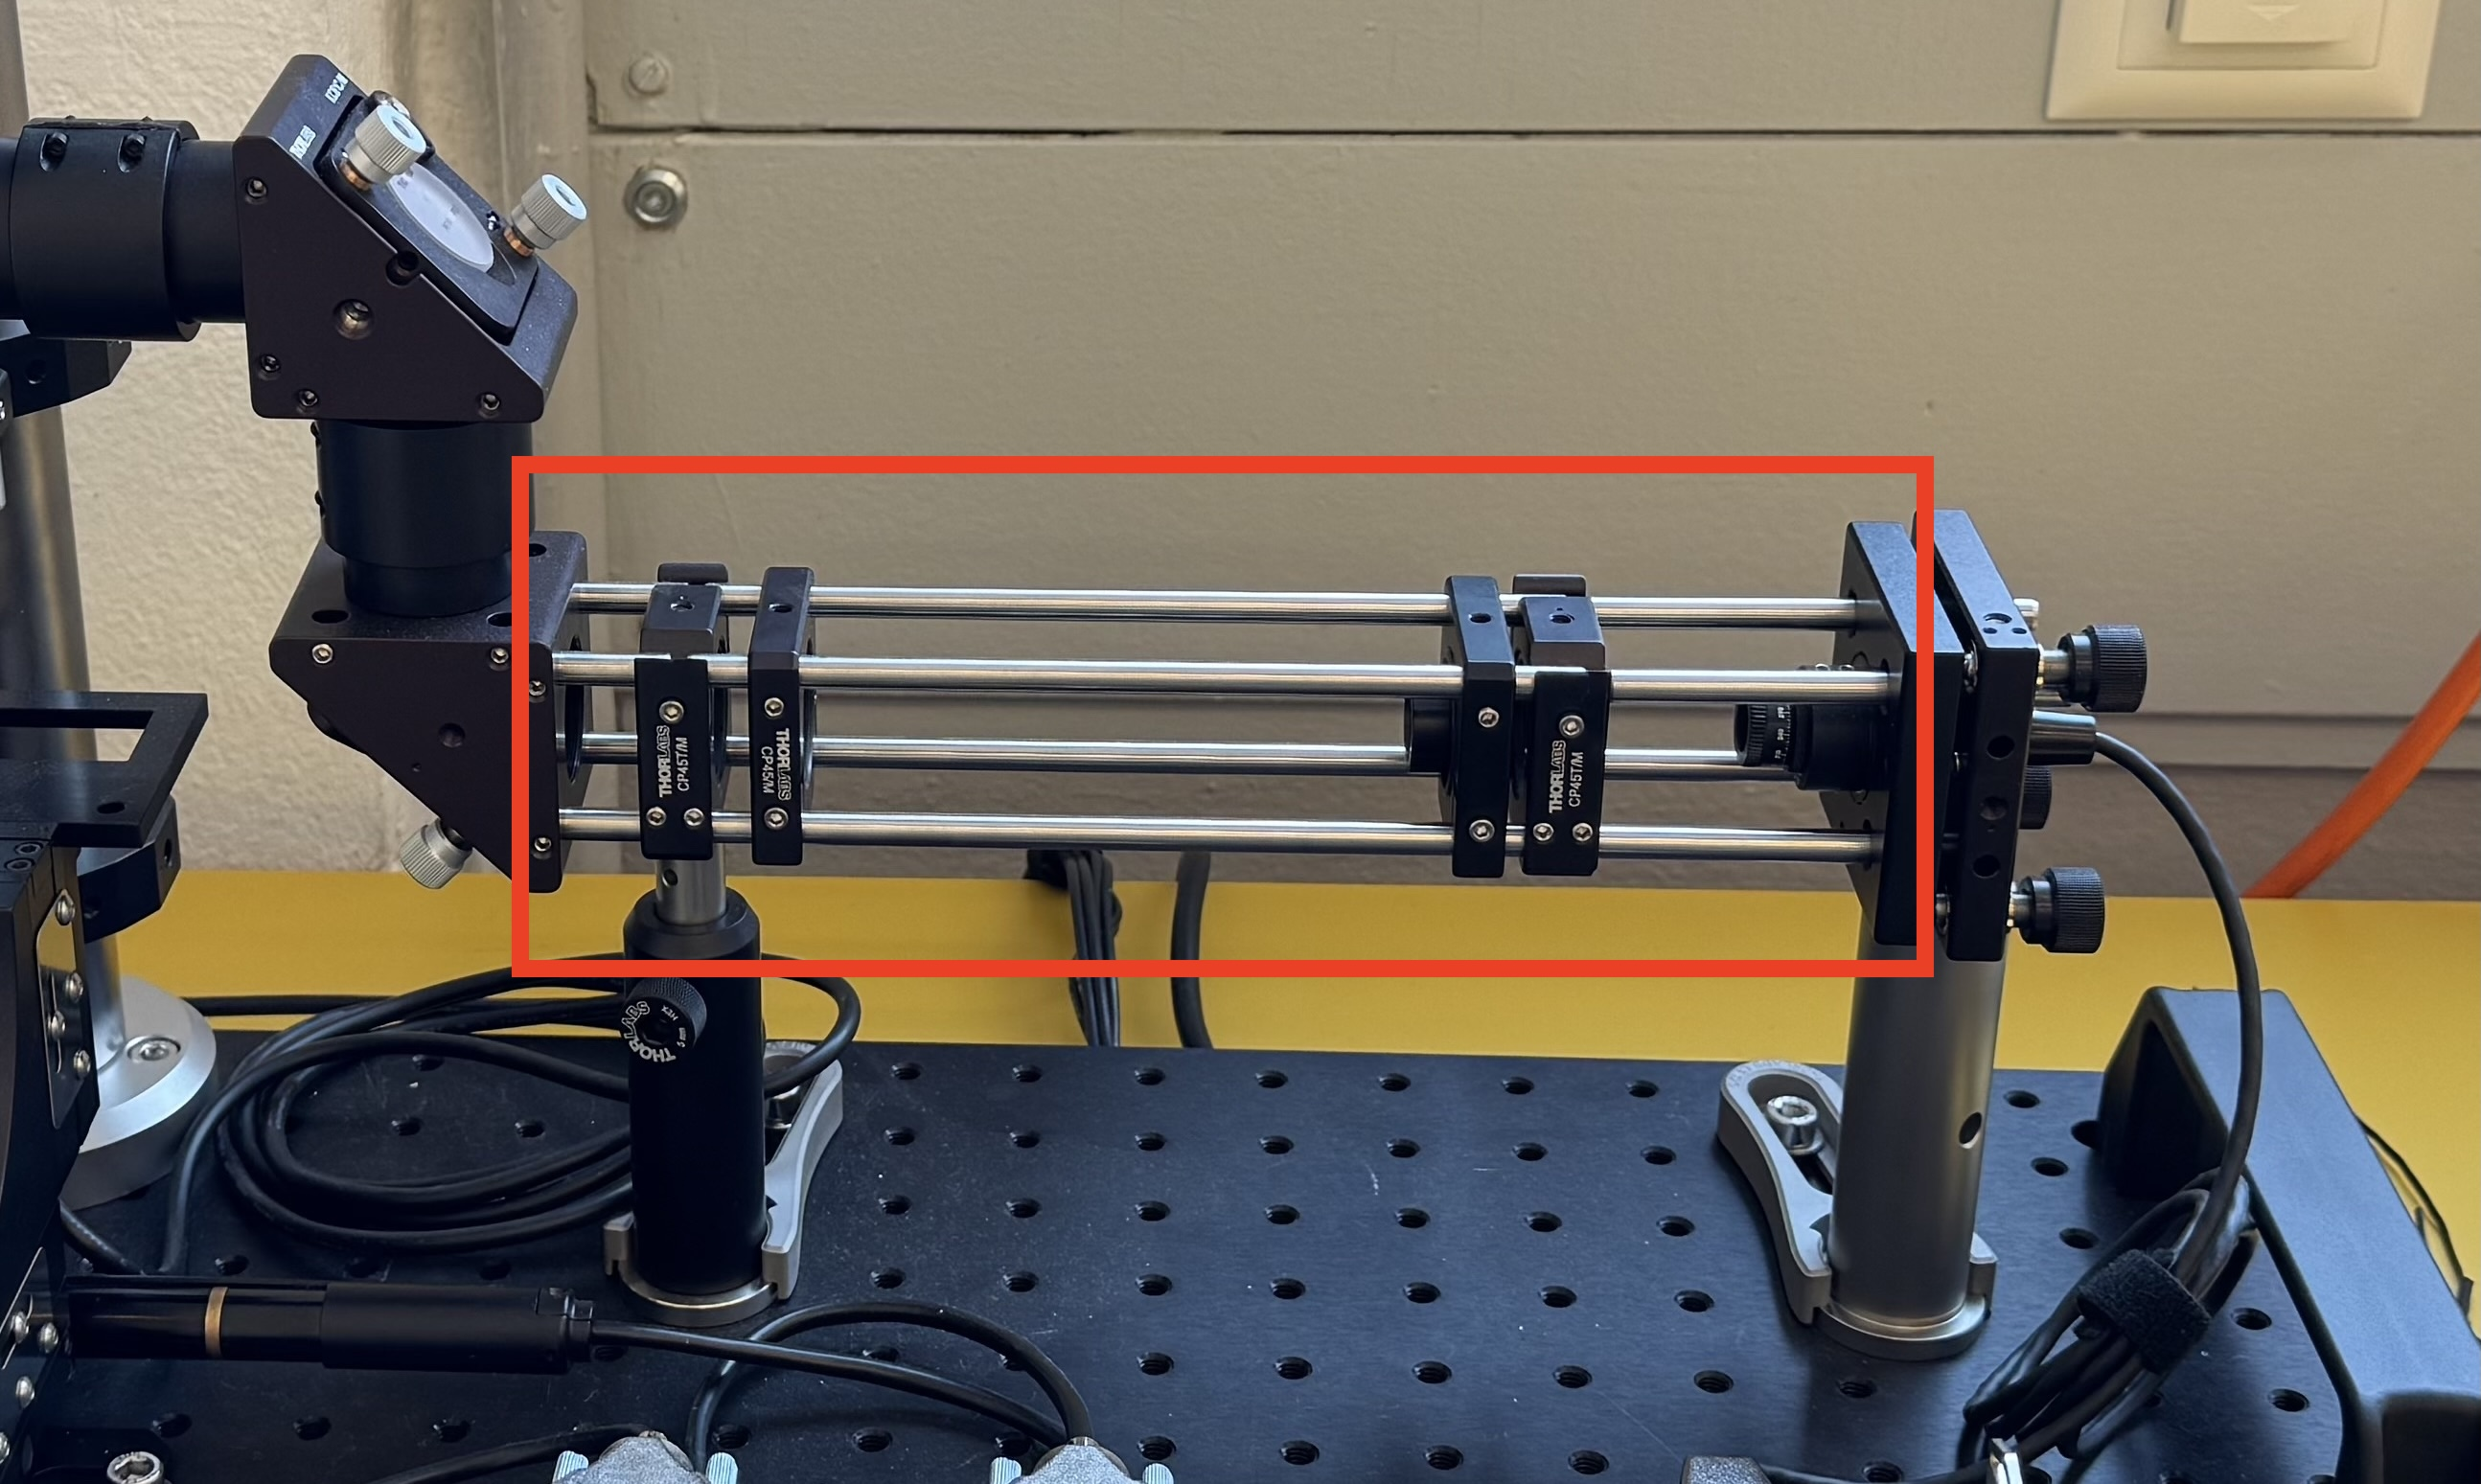
\includegraphics[width=0.5\textwidth]{assets/figures/Introduction/protection_debut_laser.jpeg}
    \end{center}
    \caption{Première protection contre le laser située vers le laser}
    \label{protection_laser_début}
\end{figure}

Une deuxième protection va être faite vers le microscope, car également à cet endroit, le laser devient visible à l'oeil nu et il y'a un grand risque de se blesser. L'encadré en \textcolor{blue}{bleu} représente l'endroit où va devoir être imaginer la protection. Voir la Figure \ref{protection_laser_fin}.

\begin{figure}[H]
    \begin{center}
        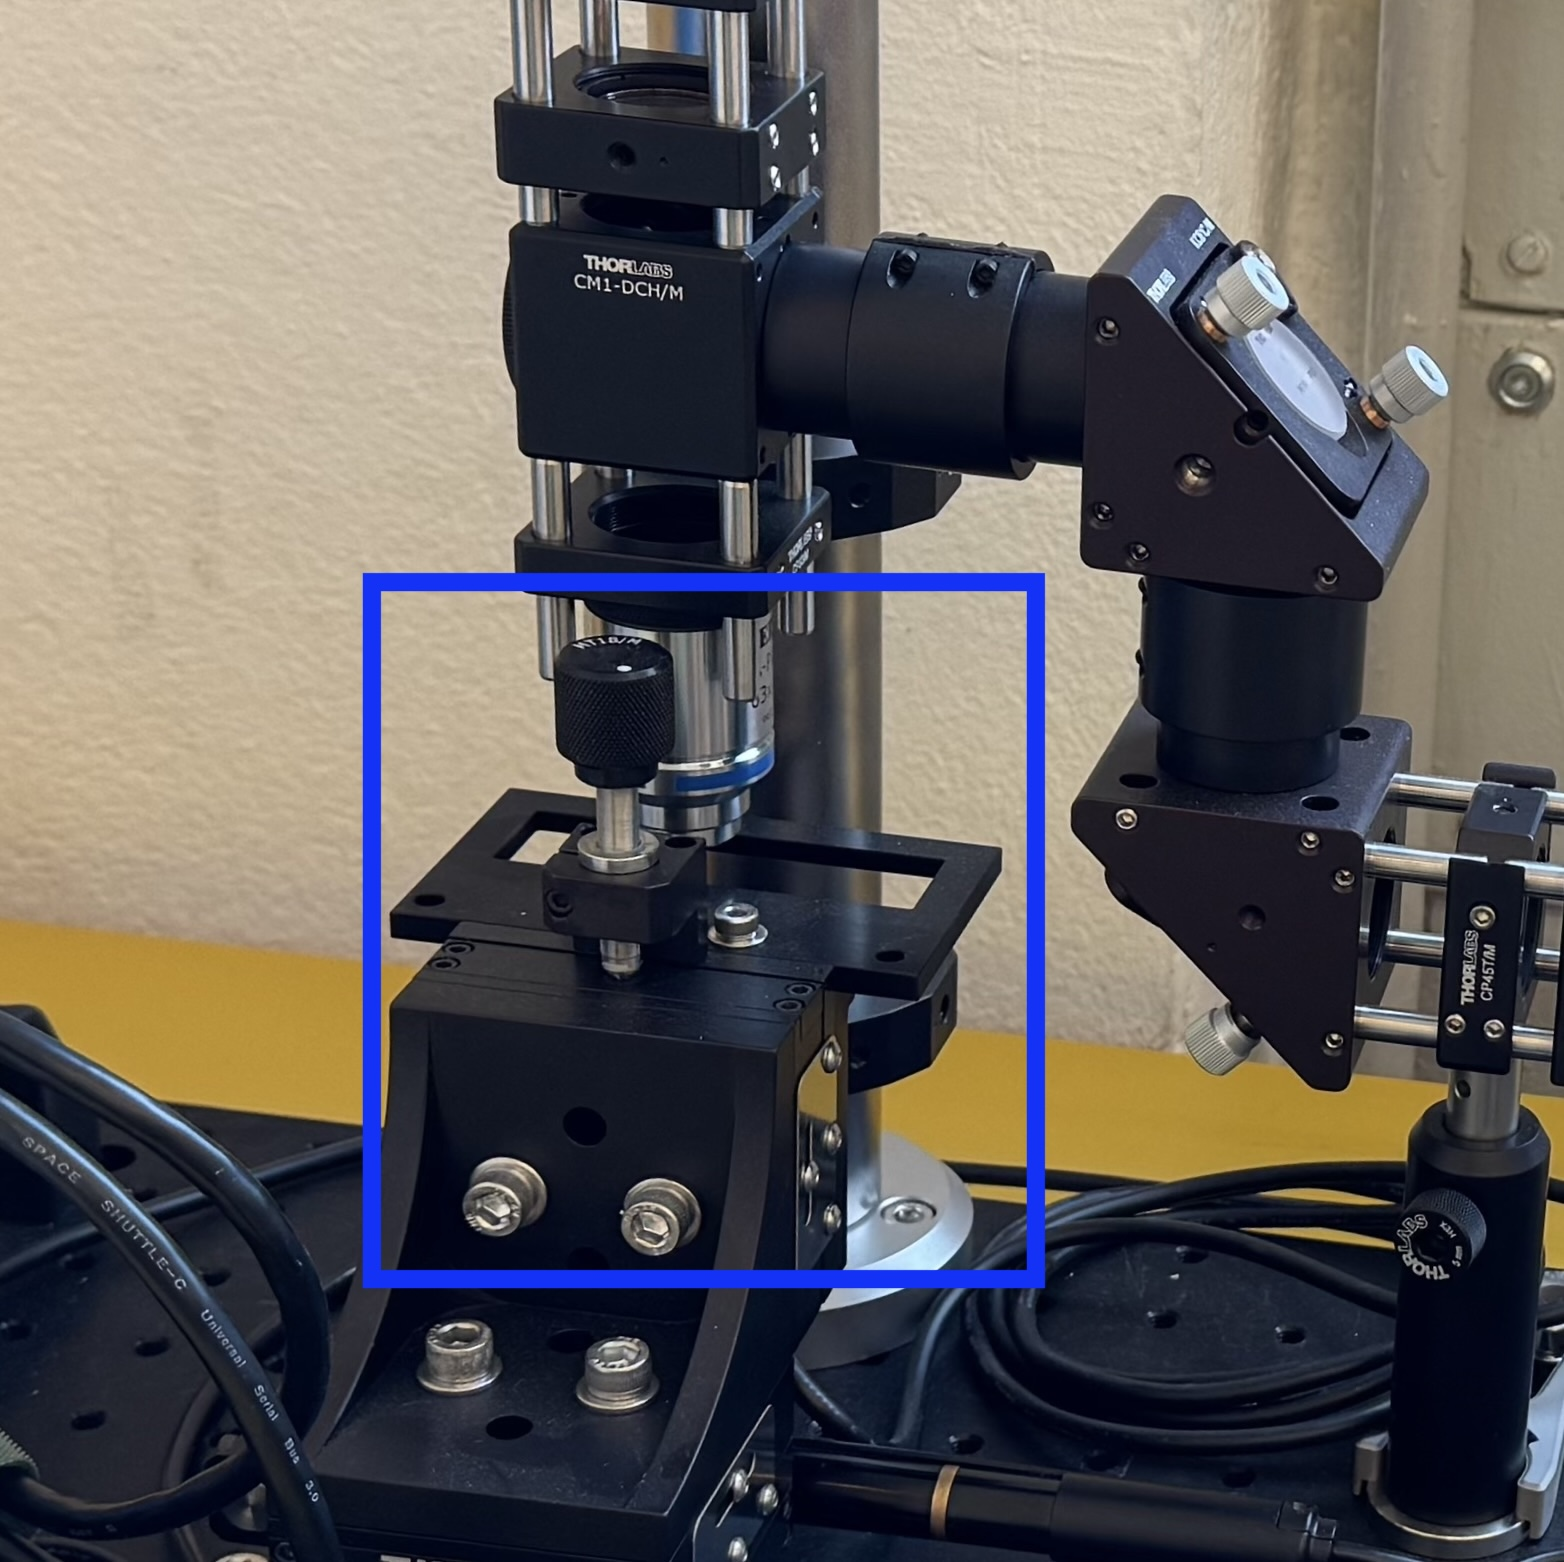
\includegraphics[width=0.5\textwidth]{assets/figures/Introduction/protection_fin_laser.jpeg}
    \end{center}
    \caption{Deuxième protection contre le laser située vers le microscope}
    \label{protection_laser_fin}
\end{figure}

\subsection{Notice de laboratoire}

Un des objectifs de ce TB, consite également à créer une notice de laboratoire pour un cours d'étudiants de la filière système industriels. Cette notice devra être simple à comprendre, compacte et comprendra des manipulations avec différents liquides, ainsi que des mesures pratiques.

%%if
\section{Citations et bibliographie}
Citer vos sources est essentiel. Avec \texttt{biblatex} vous pouvez facilement citer des articles, des livres ou des sites internet. Toutes les citations dans le texte seront automatiquement regroupées en fin de document dans la section \guillemotleft Bibliographie\guillemotright. Par exemple, citons un article d'Einstein \cite{einstein} ou le livre de Dirac \cite{dirac}.

Parfois il peut être utile d'utiliser un gestionnaire de bibliographie. La communauté académique recommande l'outil \href{https://www.zotero.org/}{Zotero} qui permet de gérer une bibliothèque numérique d'ouvrages et de références numériques. Il permet également de générer une bibliographie compatible avec \LaTeX.

Notez qu'il est très facile d'obtenir l'extrait \texttt{bibtex} depuis des journaux. Sélectionnez \emph{export/citation}. Si vous le pouvez choisissez \texttt{bibtex}. Dans le cas d'un format \texttt{.ris}, utilisez un convertisseur en ligne comme \href{http://www.bruot.org/ris2bib/}{ris2bib}.

\section{Adapter votre modèle}
Ce document n'est qu'un modèle ayant pour but de revoir les quelques avantages de \LaTeX~ et les fonctionnalités qui pourraient vous être utiles pour rédiger un rapport académique. N'hésitez pas à supprimer les parties inutiles et à adapter ce modèle à vos besoins.
%%fi
\input{examples.tex}

\chapter{Conclusion}
%%if
% Bien que non nécessaire dans un rapport de Bachelor, la discussion finale d'un projet résume les résultats obtenus et dresse une conclusion objective du projet. Un manager de société est souvent amené à lire de nombreux rapport, il ne s'intéresse généralement qu'à l'introduction au contexte de l'étude et à sa conclusion.

% Si nécessaire, n'hésitez pas à scinder votre conclusion en deux parties : une conclusion technique et une conclusion personnelle.

% Il est de coutume de signer la conclusion...
%%fi
\section*{Bilan technique}
Depuis la réception du système de pinces optiques au début du travail de bachelor, de nombreuses améliorations ont pu être réalisées.

\textbf{Sécurité} :
Le système a été optimisé pour éviter tout contact direct avec le laser. Deux protections mécaniques associées chacune à un capteur électrique ont été confectionnées afin de garantir une utilisation sécurisée du système sans protection contre le laser. La première protection, située proche du laser, est un assemblage de trois tôles en aluminium accompagné d'une charnière industrielle. Celle-ci intègre un capteur qui, lorsque la protection est ouverte, coupe l'alimentation du laser. La seconde protection, située autour du microscope et imprimée en 3D, est complétée par un capteur de fin de course qui, lui aussi, coupe le laser à la moindre ouverture. Comme dans toute installation mécano-électrique, un arrêt d'urgence a été câblé, désactivant le faisceau laser. Le système correspond ainsi à un système de classe 1, lorsqu'il est fermé. Seulement l'ajustement du chemin optique nécessite l'utilisation des lunettes de protection (en mode maintenance), c.f. chapitre~\ref{section:maintenance}.

\textbf{Ergonomie} :
Une amélioration a été faite au niveau du câblage des alimentations et des câbles de communication. Le système nécessite quatre connexions USB-A pour communiquer avec l'ordinateur. Un hub USB-A à 4 ports a donc été intégré pour que finalement, un seul câble USB-A soit à brancher sur le poste. Un bouton à clé a aussi été câblé pour pouvoir manipuler le laser plus facilement lors de la maintenance, même lorsque les protections sont ouvertes.

\textbf{Application ServoVision} :
Cette application en C\#, utilisant WPF, a été programmée en regroupant les fonctionnalités de Kinesis ainsi que de ThorCam pour faciliter l'utilisation du système. Un algorithme détectant automatiquement des particules a été implémenté. Il est également possible de déplacer automatiquement une particule sous le laser.

\textbf{Notice de laboratoire} :
Le manuel d'utilisation fourni par Thorlabs étant volumineux, une notice de laboratoire a été écrite pour une prise en main rapide du système.

\textbf{Expériences de force d'attraction de particule} :
Plusieurs expériences ont été menées avec différentes matières. Le calcul de la force de maintien maximale d'une particule de graisse avec un mélange d'eau distillée et de crème a été réalisé.

\section*{Conclusion personnelle}
Ce travail de bachelor a fait appel à plusieurs domaines : la conception mécanique pour les protections, l'électricité et le câblage pour les différents capteurs ainsi que les boutons, et la programmation de l'interface homme-machine pour l'application ServoVision. Personnellement, j'aime quand le travail que j'entreprends est varié. De mon point de vue, les objectifs ont été atteints. Le système est fonctionnel, sécurisé pour des utilisateur\(\cdot\)trices non-expert\(\cdot\)es, et comporte une application ergonomique facile d'utilisation.
\vfil
\hspace{8cm}\makeatletter\@author\makeatother\par
\hspace{8cm}\begin{minipage}{5cm}
    %%if
    % Place pour signature numérique
    \printsignature
    %%fi
\end{minipage}

\clearpage
\printbibliography

\appendix
\appendixpage
\addappheadtotoc

%%if
\chapter{Première annexe}

Les annexes n'ont pas un contenu \underline{normatif} mais \underline{descriptif}. Tout contenu annexé ne doit pas être nécessaire à la bonne compréhension du travail.

Les annexes contiennent généralement :

\begin{itemize}
    \item les dessins mécaniques (mises en plan);
    \item les schémas électriques détaillés;
    \item des photographies du projet;
    \item des scripts et des extraits de code source;
    \item des documents techniques \pex \emph{datasheet};
    \item des développements mathématiques.
\end{itemize}
\section{Sous section}
\lipsum[1]
%%fi

\let\cleardoublepage\clearpage
\backmatter

\label{glossaire}
\printnoidxglossary
\label{index}
\printindex

% Le colophon est le dernier élément d'un document qui contient des notes de l'auteur concernant la mise en page et l'édition du document : il est parfaitement optionnel.
%%if
\clearpage
\Large\textbf{Colophon :}\par\normalsize
\thispagestyle{empty}
La qualité de cet ouvrage repose que le moteur \LaTeX. La mise en page et le format sont inspirés d'ouvrages scientifiques tels que le modèle de thèse de l'EPFL et celui des publications O'Reilly.

Les mises en plan et les représentations 3D sont exportées de Autodesk Fusion 360.

% Les diagrammes et les illustrations sont édités depuis l'outil en ligne draw.io. Certaines illustrations ont été reprises dans Adobe Illustrator. Les représentations 3D sont exportées de SolidWorks et certains graphiques sont générés à la volée depuis un code source Python.

% L'auteur fictive de ce document \emph{Maria Bernasconi} est un nom emprunté, par amusement, aux spécimens publiés par Postfinance.

Ce document a été compilé avec XeLaTeX.

La famille de police de caractères utilisée est \emph{Computed Modern} créée par Donald Knuth avec son logiciel METAFONT.
\vfil
% Le Colophon est le dernier élément d'un document qui contient des notes de l'auteur concernant la mise en page et l'édition du document : il est parfaitement optionnel.
%%fi

\end{document}
